% Created 2024-02-23 Fri 12:51
% Intended LaTeX compiler: pdflatex
\documentclass[presentation]{beamer}
\usepackage[utf8]{inputenc}
\usepackage[T1]{fontenc}
\usepackage{graphicx}
\usepackage{longtable}
\usepackage{wrapfig}
\usepackage{rotating}
\usepackage[normalem]{ulem}
\usepackage{amsmath}
\usepackage{amssymb}
\usepackage{capt-of}
\usepackage{hyperref}
\mode<beamer>{\usetheme{Madrid}}
\definecolor{SUred}{rgb}{0.59375, 0, 0.17969} % SU red (primary)
\definecolor{SUblue}{rgb}{0, 0.17578, 0.38281} % SU blue (secondary)
\setbeamercolor{palette primary}{bg=SUred,fg=white}
\setbeamercolor{palette secondary}{bg=SUblue,fg=white}
\setbeamercolor{palette tertiary}{bg=SUblue,fg=white}
\setbeamercolor{palette quaternary}{bg=SUblue,fg=white}
\setbeamercolor{structure}{fg=SUblue} % itemize, enumerate, etc
\setbeamercolor{section in toc}{fg=SUblue} % TOC sections
% Override palette coloring with secondary
\setbeamercolor{subsection in head/foot}{bg=SUblue,fg=white}
\setbeamercolor{date in head/foot}{bg=SUblue,fg=white}
\institute[SU]{Shenandoah University}
\titlegraphic{\includegraphics[width=0.5\textwidth]{\string~/Documents/suLogo/suLogo.pdf}}
\usepackage{tikz}
\usetheme{default}
\author{Chase Mathison\thanks{cmathiso@su.edu}}
\date{27 February 2024}
\title{Trigonometric substitution}
\hypersetup{
 pdfauthor={Chase Mathison},
 pdftitle={Trigonometric substitution},
 pdfkeywords={},
 pdfsubject={},
 pdfcreator={Emacs 29.1 (Org mode 9.6.7)}, 
 pdflang={English}}
\begin{document}

\maketitle

\section{Announcements}
\label{sec:orgc54cb3b}
\begin{frame}[label={sec:org93365d3}]{Announcements}
\begin{enumerate}
\item Don't forget about exam corrections!
\item Homework assigned in MyOpenMath.
\item Office hours M-F, 10am - 11am
\end{enumerate}
\end{frame}

\section{The Lecture}
\label{sec:org527bc78}
\begin{frame}[label={sec:orgda24b62}]{Trig substitution, why do we need it?}
Today we will finally learn how to find an antiderivative of the
function
\[
\sqrt{1-x^2}. \]
Integrating functions that involve \(\sqrt{a^2-x^2}\) is one of the
key motivations for developing trigonometric substitution.

We'll also use trigonometric substitution to integrate functions that
involve \(\sqrt{x^2-a^2}\) and \(\sqrt{a^2 + x^2}.\) So almost
anytime that we deal with integrating a function that has one of these
three forms in it, you can pretty safely bet that trigonometric
substitution will be involved.
\end{frame}

\begin{frame}[label={sec:org43c7a18}]{A reminder: SOHCAHTOA}
\begin{center}
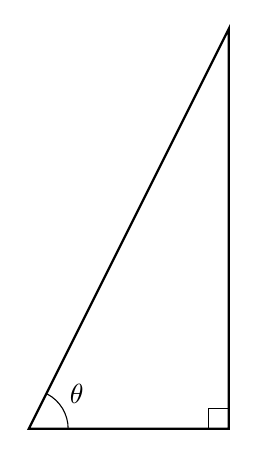
\begin{tikzpicture}
\draw[thick] (0,0) -- ++(0:1in) -- ++(90:2in) -- cycle;
\draw (0.5,0) arc (0:62:0.5cm);
\draw (0,0) ++(31:0.6cm) node[above right,inner sep=0] {\(\theta \)};
\draw (1in,0) rectangle (0.9in,0.1in);
\end{tikzpicture}
\end{center}
\end{frame}

\begin{frame}[label={sec:org83b64cd}]{The idea}
I'll illustrate the main idea for integrating functions that involve
\(\sqrt{a^2-x^2}\) with the following example.
\[\int\limits_{}^{} \sqrt{1-x^2}\,dx \]
\vspace{10in}
\end{frame}

\begin{frame}[label={sec:org55e5046}]{Integrals involving \(\sqrt{a^2-x^2}\)}
In general, to integrate a function that involves \(\sqrt{a^2-x^2}\),
use the following strategy:
\begin{center}
\includegraphics[width=0.8\textwidth]{../img/trigSub1.png}
\end{center}
\end{frame}

\begin{frame}[label={sec:org415b5be}]{Example}
Evaluate
\[\int\limits_{}^{} \frac{x^2}{\sqrt{4-x^2}}\,dx \]
\vspace{10in}
\end{frame}

\begin{frame}[label={sec:org120ea72}]{Example}
Evaluate
\[
\int\limits_0^{\frac{1}{2}} \frac{1}{1-x^2}\,dx \]
\vspace{10in}
\end{frame}

\begin{frame}[label={sec:org0ead5af}]{Example}
\end{frame}

\begin{frame}[label={sec:org3c0208b}]{Integrals involving \(\sqrt{a^2+x^2}\)}
Integrating functions that involve \(\sqrt{a^2+x^2}\) works in a very
similar way, we just need to make a slightly different trigonometric
substitution:

\begin{center}
\includegraphics[width=0.8\textwidth]{../img/trigSub2f.png}
\end{center}
\end{frame}

\begin{frame}[label={sec:orga1d8898}]{Example}
Evaluate
\[
\int\limits_{}^{} \frac{1}{\sqrt{3+x^2}}\,dx \]
\vspace{10in}
\end{frame}

\begin{frame}[label={sec:orgc8b0c67}]{Example}
\end{frame}
\end{document}